% Source of vignettes/figures/strata_data.png, taken from the earlier PDF version of the vignette.
% Rendered with vignettes/figures-src/render.sh (pdflatex, pdfcrop, Ghostscript).
\documentclass{article}
\usepackage[margin=1in,paperwidth=8.5in,paperheight=11in]{geometry} % text width as in the PDF vignette
\usepackage{xcolor}
%\PassOptionsToPackage{svgnames}{xcolor}


\usepackage{amsmath,bbm,amssymb}
\usepackage{bm}
\usepackage{amsthm}
%\usepackage{xcolor}
% natbib is not loaded: citations are processed by pandoc (citeproc), and
% natbib's author-year check failed on CRAN (archived 2023-09-21)

\usepackage[eulergreek]{sansmath}
\usepackage{tikz} % for venn diagrams
\usetikzlibrary{shapes,backgrounds,shapes.misc,decorations.pathreplacing, positioning,shapes.geometric,arrows,matrix,fit,calc,arrows.meta, trees, hobby}
\usepackage[outline]{contour}
\contourlength{0.5pt}

\definecolor{DimGray}{rgb}{0.75, 0.75, 0.75}

\newcommand{\bmath}[1]{\mbox{ \boldmath $\!#1\!$ \unboldmath}}
\newcommand{\alert}[1]{\textcolor{red}{\!#1\!}}

\tikzset{
    buffer/.style={
        isosceles triangle,
        isosceles triangle apex angle=66,
        shape border rotate=90,
        draw,
        thick,
        fill=blue!20,
        node distance=5cm,
        rounded corners=60pt,
        opacity=0.6,
        minimum height=6.25cm
    }
}

\pgfdeclarelayer{foreground}
\pgfdeclarelayer{background}
   \pgfsetlayers{background,%
                 main,%
                 foreground%
                 }

\def\v{\mathbf}
\def\m{\boldsymbol}
\def\vb{\bm{\upbeta}}\def\ve{\bm{\upvarepsilon}}\def\vg{\bm{\upgamma}}\def\vl{\bm{\uplambda}}\def\vp{\bm{\upphi}}\def\vpsi{\bm{\uppsi}}\def\vpi{\bm{\uppi}}
\def\vt{\bm{\uptheta}}\def\vx{\bm{\upxi}}\def\vd{\bm{\updelta}}\def\va{\bm{\upalpha}}
\def\coef{\boldsymbol \beta}
\def\hcoef{\hat{\boldsymbol \beta}}
\def\bbeta{\boldsymbol \beta}
\def\bgamma{\boldsymbol \gamma}
\def\bnu{\boldsymbol \nu}
\def\boldeta{\boldsymbol \eta}
\def\betahat{\hat{\boldsymbol \beta}}
\def\betatrue{\boldsymbol \beta^0}
\def\coeftheta{\boldsymbol \theta}
\def\hcoeftheta{\hat{\boldsymbol \theta}}
\def\hbeta{\hat{\beta}}
\def\bfy{\mathbf y}
\def\bfY{\mathbf Y}
\def\bfF{\mathbf F}
\def\bfu{\mathbf u}
\def\bfX{\mathbf X}
\def\bfZ{\mathbf Z}
\def\bfW{\mathbf W}
\def\bfx{\mathbf x}
\def\bfu{\mathbf u}
\def\bfzero{\mathbf 0}
\def\bzero{\boldsymbol 0}
\def\bfg{\mathbf g}
\def\bQ{\boldsymbol Q}
\def\bfQ{\mathbf Q}
\def\blnorm{\biggr\lVert}
\def\brnorm{\biggr\lVert}
\def\bfI{\mathbf I}
\def\bfM{\mathbf M}
\def\bfT{\mathbf T}

\def\P{\mathrm{P}}
\def\E{\mathrm{E}}
\def\V{\mathrm{Var}}
\def\Cov{\mathrm{Cov}}
\def\cor{\mathrm{Corr}}
\def\d{\mathrm{d}}
\pagestyle{empty}
\begin{document}
\begin{center}

\resizebox{.75\textwidth}{!}{% <------ Don't forget this %
\tikzstyle{background rectangle}=
[draw=blue!8,fill=blue!8,rounded corners=1.5ex]
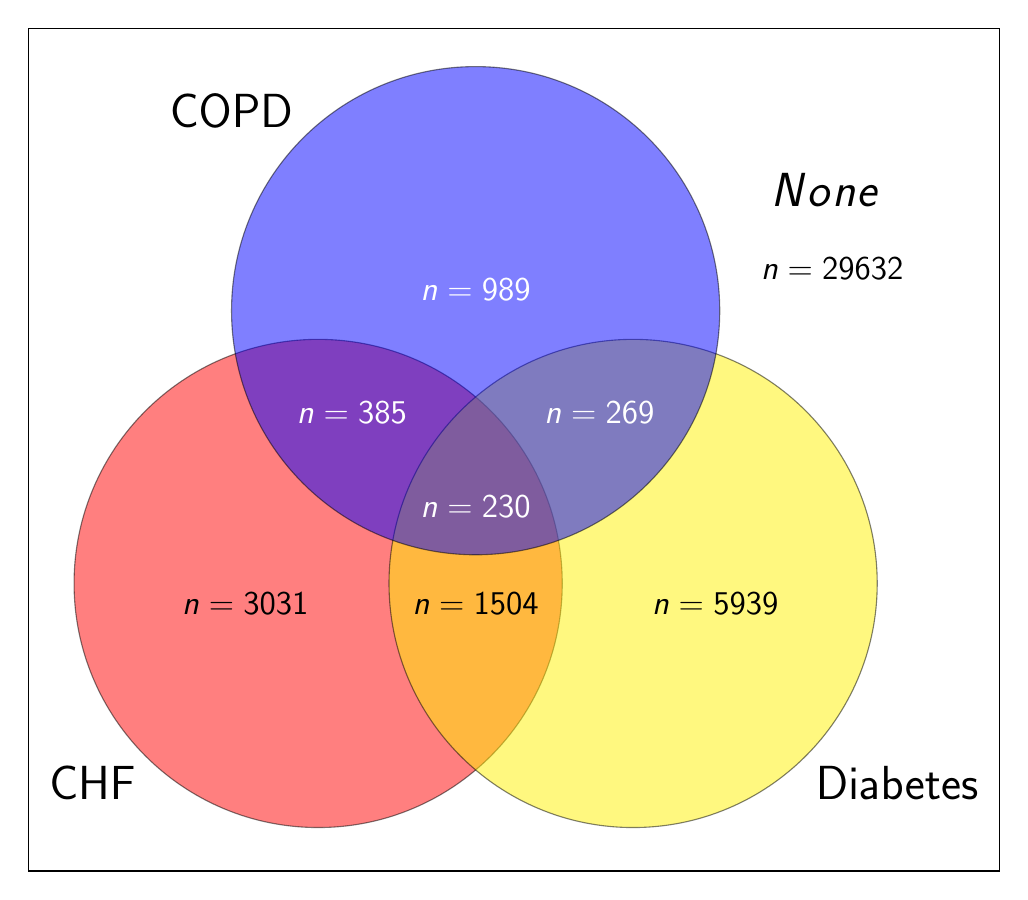
\begin{tikzpicture}[font=\sffamily\sansmath,show background rectangle]
% \node (1) [draw, rounded rectangle] {none};
  \tikzset{venn circle/.style={draw,circle,minimum width=6.2cm,fill=#1,opacity=0.5}}

  \node [venn circle = red][label=below left:{\LARGE CHF}] (A) at (0,0) {\large {}};
  \node [venn circle = yellow][label=below right:{\LARGE Diabetes}] (C) at (0:4cm) {\large {}};
  \node [venn circle = blue][label=above left:{\LARGE COPD}] (B) at (60:4cm) {\large {}};
  \node[left,text=white] at (barycentric cs:A=0.9/3,B=1/2 ) {\large $n = 385$}; %
  \node[below] at (barycentric cs:A=1/2,C=1/2 ) {\large $n = 1504$};   %
  \node[right,text=white] at (barycentric cs:B=1/2,C=0.9/3 ) {\large $n = 269$};   %
  \node[below,text=white] at (barycentric cs:A=0.9/3,B=1/3,C=0.9/3 ){\large $n = 230$};%
  \node[below left] at (A.center) {{\large $n=3031$}}; %
  \node[below right] at (C.center)  {{ \large $n = 5939$}}; %
  \node[above,text=white] at (B.center) {{\large $n = 989$}};  %





  \node[label=right:\LARGE$None$ ] (Non) at (5.5,5)  {}; 
  \node[right] at (5.5,4) {{\large $n = 29632$}};  

  %\draw[thick,green]  (-3.5,0) --(7.5,0);
  %\draw[thick,green]  (0,-3.5) --(0,6.9);

  \path(-3.5,0) --(7.5,0);
  \path(0,-3.5) --(0,6.9);
\end{tikzpicture}
}


\end{center}
\end{document}
